\documentclass[tikz,border=6pt]{standalone}
\usepackage{fontspec}
\setmainfont{Noto Sans}
\usepackage{amsmath,amssymb}
\usepackage{tikz}
\usetikzlibrary{arrows.meta,positioning,shapes.geometric,fit,calc}

\definecolor{cudaG}{RGB}{118,185,0}
\definecolor{sadRed}{RGB}{200,60,50}
\definecolor{gsBlue}{RGB}{40,110,190}
\definecolor{pyYel}{RGB}{240,170,30}
\definecolor{greyT}{RGB}{85,85,85}

\begin{document}
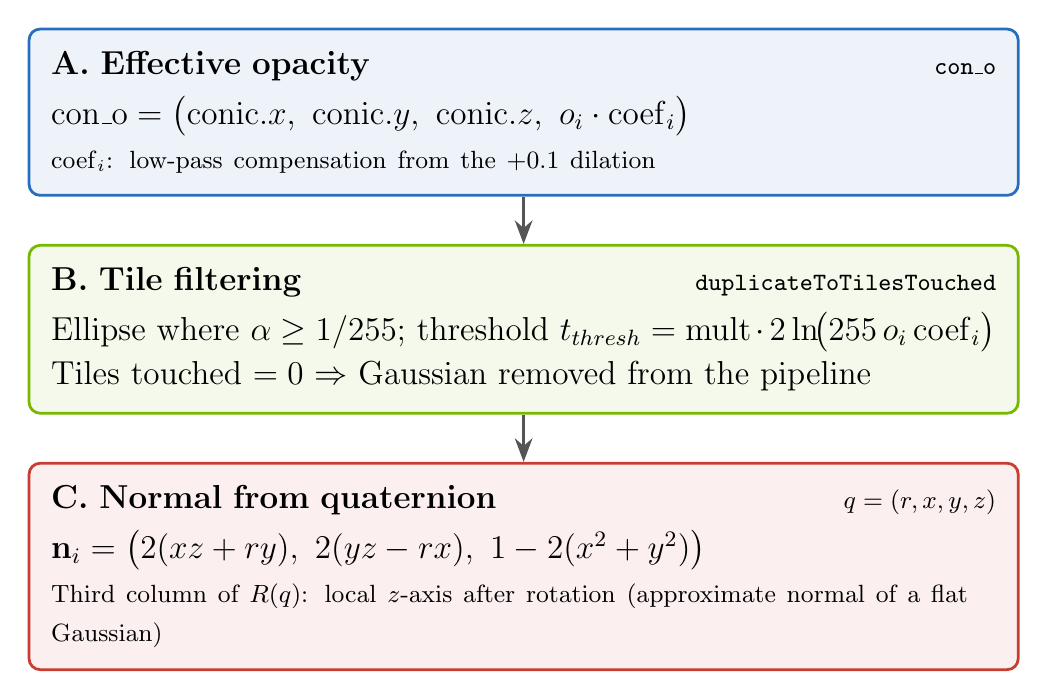
\begin{tikzpicture}[
  step/.style={draw=#1, line width=1pt, rounded corners, fill=#1!8,
    align=left, inner sep=8pt, text width=12cm, font=\large},
  lab/.style={font=\bfseries\large, text=#1},
  arr/.style={-{Stealth[length=3mm]}, line width=1pt, greyT},
]

% Step A: effective opacity
\node[step=gsBlue] (A) {%
  \textbf{A. Effective opacity} \hfill {\small \texttt{con\_o}}\\[4pt]
  $\mathrm{con\_o}=\bigl(\mathrm{conic}.x,\ \mathrm{conic}.y,\ \mathrm{conic}.z,\ o_i\cdot\mathrm{coef}_i\bigr)$\\[2pt]
  {\small $\mathrm{coef}_i$: low-pass compensation from the $+0.1$ dilation}};

% Step B: tile filtering
\node[step=cudaG, below=0.6cm of A] (B) {%
  \textbf{B. Tile filtering} \hfill {\small \texttt{duplicateToTilesTouched}}\\[4pt]
  Ellipse where $\alpha \ge 1/255$; threshold $t_{thresh}=\mathrm{mult}\cdot 2\ln\!\bigl(255\,o_i\,\mathrm{coef}_i\bigr)$\\[2pt]
  Tiles touched $=0$ $\Rightarrow$ Gaussian removed from the pipeline};

% Step C: normal from quaternion
\node[step=sadRed, below=0.6cm of B] (C) {%
  \textbf{C. Normal from quaternion} \hfill {\small $q=(r,x,y,z)$}\\[4pt]
  $\mathbf n_i=\bigl(2(xz+ry),\ 2(yz-rx),\ 1-2(x^2+y^2)\bigr)$\\[2pt]
  {\small Third column of $R(q)$: local $z$-axis after rotation (approximate normal of a flat Gaussian)}};

\draw[arr] (A) -- (B);
\draw[arr] (B) -- (C);

\end{tikzpicture}
\end{document}
